%%%%%%%%%%%%%%%%%%%%%%%%%%%%%%%%%%%%%%%%%
% Uppsala University Assignment Title Page 
% LaTeX Template
% Version 1.0 (27/12/12)
%
% This template has been downloaded from:
% http://www.LaTeXTemplates.com
%
% Original author:
% WikiBooks (http://en.wikibooks.org/wiki/LaTeX/Title_Creation)
% Modified by Elsa Slattegard to fit Uppsala university
% License:
% CC BY-NC-SA 3.0 (http://creativecommons.org/licenses/by-nc-sa/3.0/)

%\title{Title page with logo}
%----------------------------------------------------------------------------------------
%	PACKAGES AND OTHER DOCUMENT CONFIGURATIONS
%----------------------------------------------------------------------------------------

\documentclass[12pt]{article}
\usepackage[english]{babel}
\usepackage[utf8x]{inputenc}
\usepackage{amsmath}
\usepackage{amssymb}
\usepackage{graphicx}
\usepackage{caption}
\usepackage{subcaption}
\usepackage{float}
\usepackage{tabularx}
\usepackage{booktabs}
\usepackage{tabularray}
\usepackage{tabularray}
\usepackage{ragged2e}
\usepackage{multicol}
\usepackage{multirow}
\usepackage{hyperref}
\usepackage{microtype}
\usepackage[colorinlistoftodos]{todonotes}
\usepackage[ruled,vlined]{algorithm2e}
\usepackage{cite}

\setlength {\marginparwidth }{2cm}

\begin{document}
    \begin{titlepage}
    
    \newcommand{\HRule}{\rule{\linewidth}{0.5mm}} % Defines a new command for the horizontal lines, change thickness here
    
    \center % Center everything on the page
     
    %----------------------------------------------------------------------------------------
    %	HEADING SECTIONS
    %----------------------------------------------------------------------------------------
    
    \textsc{\LARGE{T\'{e}cnico Lisboa} \\ \vspace{0.5cm} \LARGE{University of Lisbon}}\\[1cm] % Name of your university/college
    \vspace{-2cm}
    \begin{figure}[H]
        \centering
        \begin{minipage}{.5\textwidth}
            \centering
            \phantom{............}
\includegraphics[width=.9\linewidth]{figures/logos/university-lisbon-logo.png}
        \end{minipage}%
        \begin{minipage}{.5\textwidth}
            \centering
            \hspace{-1cm}
            
\includegraphics[width=.9\linewidth]{figures/logos/tecnico-ulisboa-logo.png}
        \end{minipage}
    \end{figure}
    \vspace{-1cm}
     % Include a department/university logo - this will require the graphicx package
    \textsc{\Large Research Seminar in Information Security}\\[0.5cm] % Major heading such as course name
    \textsc{(Prof. Paulo \uppercase{Mateus})}\\[0.5cm]
    \textsc{Doctoral Program in Information Security}\\[0.5cm] % Minor heading such as course title
    \textsc{\large 2023/2024 - 1\textsuperscript{st} Semester}\\[0.5cm] % Minor heading such as course title
    
    %----------------------------------------------------------------------------------------
    %	TITLE SECTION
    %----------------------------------------------------------------------------------------
    
    \HRule \\[0.3cm]
        { \huge \bfseries Quantum Protocols for Secure Multi-Party Computation:\\ \Large From Theory to Practice \\ \vspace{0.5cm} \Large (Alex \textsc{\uppercase{Grilo}} - November 23, 2023)}\\[0.4cm] % Title of your document
    \HRule \\[1cm]
     
    %----------------------------------------------------------------------------------------
    %	AUTHOR SECTION
    %----------------------------------------------------------------------------------------
    
    \begin{minipage}{0.75\textwidth}
    
        \begin{flushleft} \large
            \textbf{Report written by:}\\
            \begin{itemize}
                \vspace{-0.1cm}
                \item \normalsize{Rúben \textsc{\uppercase{Barreiro}}:\\
                - \href{mailto:ruben.andre.letra.barreiro@tecnico.ulisboa.pt}{\emph{ruben.andre.letra.barreiro@tecnico.ulisboa.pt}}}
            \end{itemize}
        \end{flushleft}
    
    \end{minipage}\\[2cm]
    \vspace{-1cm}    
    % If you don't want a supervisor, uncomment the two lines below and remove the section above
    %\Large \emph{Author:}\\
    %John \textsc{Smith}\\[3cm] % Your name
    
    %----------------------------------------------------------------------------------------
    %	DATE SECTION
    %----------------------------------------------------------------------------------------
    
    {\large{Last updated: \today}}\\[2cm] % Date, change the \today to a set date if you want to be precise
    
    \vfill % Fill the rest of the page with whitespace

    \end{titlepage}

    \clearpage

    \section{Motivation}
    \label{sec:motivation}

    The task of interest in this seminar is to address how to use quantum\break properties to have Secure Multi-Party Computation (SMPC) protocols\break \cite{shamir-rivest-adleman:mental-poker:1981:03-2024,yao:protocols-secure-computations:1982:03-2024,yao:how-generate-and-exchange-secrets:1986:03-2024,goldreich-micali-wigderson:how-play-any-mental-game-completeness-theorem-protocols-honest-majority:1987:03-2024,ben-or-goldwasser-wigderson:completeness-theorems-non-cryptographic-fault-tolerant-distributed-computation:1988:03-2024,chaum-crepeau-damgard:multiparty-unconditionally-secure-protocols:1988:03-2024}, from the theoretical to the practical side. First, we need to define\break the appropriate scenario for an SMPC protocol before entering into the deep details of this seminar. In these protocols, we have multiple $N$ parties, and each one of them has some input data $\vec{x} = ({x}_{1}, {x}_{2}, ..., {x}_{N})$. Then, they jointly want to compute an abstract function $f$ on these mentioned input data.\break However, they do not want to reveal the respective information like that data\break itself. These SMPC protocols are one of the most general and fundamental\break cryptographic primitives if we do not know the number of rounds or how much communication we will need. So, ideally, in these protocols, we have a trusted party or a trusted node to which every other party can send their input data and information. This trusted node would compute the output\break data for the function $f$ and send back this value to every other party or node. 

    \begin{figure}[ht]
        \captionsetup{justification=centering}
        \centering
        \begin{subfigure}{.33\textwidth}
            \centering
            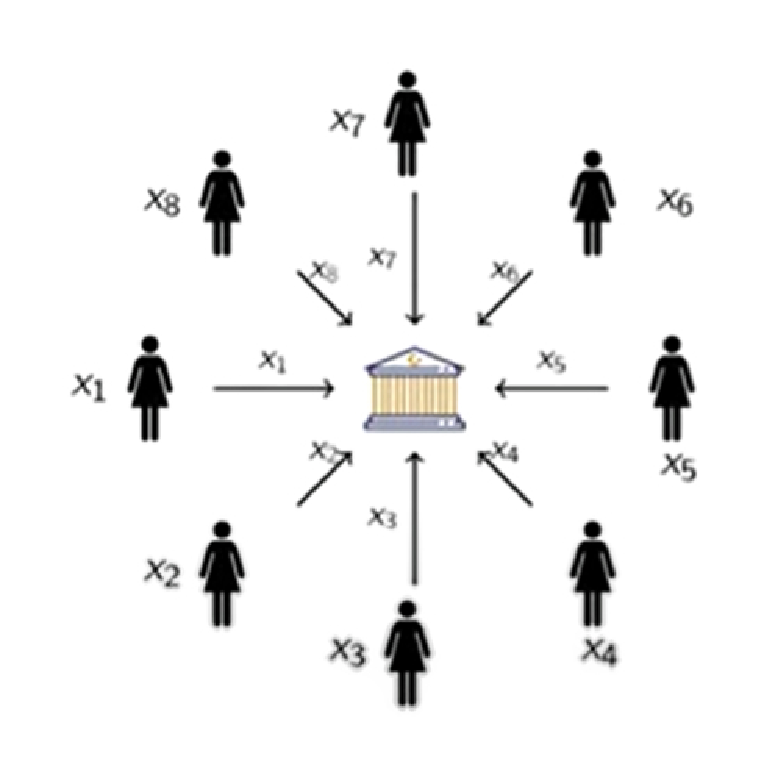
\includegraphics[width=\linewidth]{figures/images/img-1.pdf}
            \caption{Each one of\\ the $N$ parties has\\ some input data\\ $\vec{x} = ({x}_{1}, {x}_{2}, ..., {x}_{N})$\\ and send it to a\\ ``central'' trusted party.}
            \label{fig:secure-multi-party-computation-protocol-step-1}
        \end{subfigure}%
        \begin{subfigure}{.33\textwidth}
            \centering
            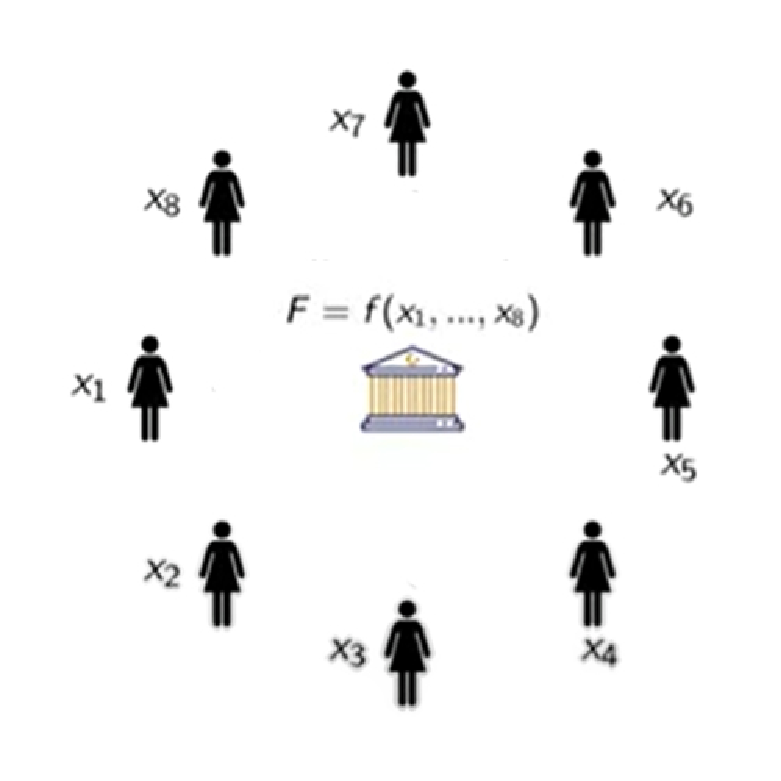
\includegraphics[width=\linewidth]{figures/images/img-2.pdf}
            \caption{The ``central'' trusted\\ \phantom{.....} party computes an\\ arbitrary function $f$\\ on the input data\\  $\vec{x} = ({x}_{1}, {x}_{2}, ..., {x}_{N})$.\\ \phantom{.}}
            \label{fig:secure-multi-party-computation-protocol-step-2}
        \end{subfigure}%
        \begin{subfigure}{.33\textwidth}
            \centering
            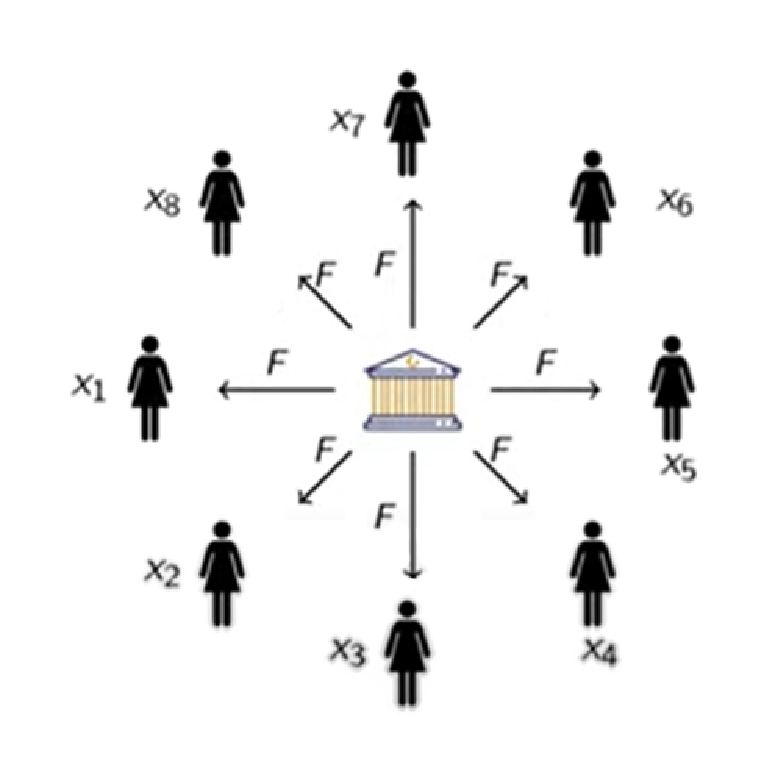
\includegraphics[width=\linewidth]{figures/images/img-3.pdf}
            \caption{The ``central'' trusted\\ party send back\\ the output result of\\ the function $f$ on\\ the input data\\ $\vec{x} = ({x}_{1}, {x}_{2}, ..., {x}_{N})$.}
            \label{fig:secure-multi-party-computation-protocol-step-3}
        \end{subfigure}
        \caption{High-level illustration of the usual steps involved in\\ a Secure Multi-Party Computation (SMPC) protocol.}
        \label{fig:secure-multi-party-computation-protocol-steps}
    \end{figure}
    
    \noindent Therefore, we trust this ``central'' node would not reveal the information\break concerning that function or the input data. This function $f$ can reveal some information about the input data, but the goal is that it does not disclose more than the output data of that function $f$. Hence, this is the most that a party can ideally learn about the other parties' input data. However, the problem is we do not live in the ideal world but in the real world. Thus, we want to implement this functionality without the previously\break mentioned ``central'' trusted node. In that direction, we want a protocol where the parties interact and communicate with each other, and eventually,\break some of these parties are malicious. For example, they could want to deviate\break from the protocol to learn the input data of a single honest party.\break Then, the goal is to ensure that the function $f$ is the only thing they are able to learn, even if some parties collude and behave dishonestly, trying to obtain as much information as they want from a single honest party.

   \begin{figure}[ht]
        \captionsetup{justification=centering}
        \centering
        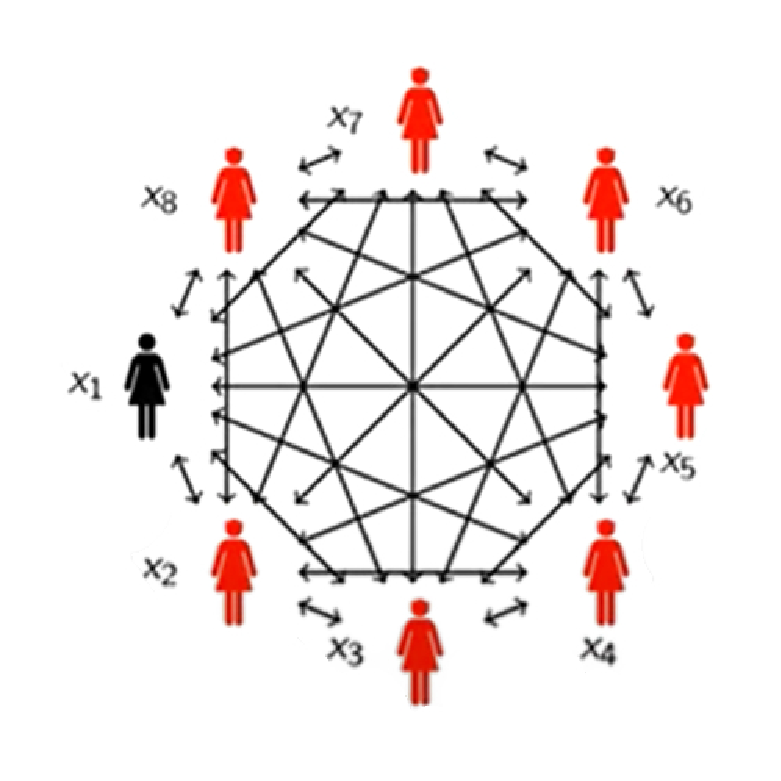
\includegraphics[width=0.4\textwidth]{figures/images/img-4.pdf}
        \caption{High-level illustration of a Secure Multi-Party\\ Computation (SMPC) protocol, with malicious/dishonest parties.}
    \end{figure}

    \noindent In Classical Cryptography, there are two principal families of SMPC\break protocols, and both of them rely on information-theoretic security (also called unconditional security), known as Goldreich-Micali-Wigderson (GMW) \cite{goldreich-micali-wigderson:how-play-any-mental-game:1987:03-2024} and Ishai-Prabhakaran-Sahai (IPS) \cite{ishai-prabhakaran-sahai:founding-cryptography-oblivious-transfer-efficiently:2008:03-2024} families/paradigms. The former are SMPC protocols from honest SMPC based on ideal Zero-Knowledge Proofs (ZKPs) \cite{goldwasser-micali-rackoff:1985:03-2024,fiat-shamir:how-prove-yourself-practical-solutions-identification-signature-problems:1987:03-2024,blum-feldman-micali:non-interactive-zero-knowledge-applications:1988:03-2024}, and the latter are SMPC protocols from honest SMPC based\break on ideal Oblivious Transfers (OTs) \cite{rabin:how-exchange-secrets-oblivious-transfer:1981:03-2024,even-goldreich-lempel:randomized-protocol-signing-contracts:1985:03-2024,crepeau:equivalence-between-two-flavours-oblivious-transfers:1988:03-2024,kilian:founding-cryptography-oblivious-transfer:1988:03-2024}. Both families/paradigms rely on,\break for example, the property of the majority of the parties participating in\break the protocols are malicious and dishonest. Nevertheless, by the majority, we do not mean that there is necessarily only one honest party. Furthermore, these families can rely on much stronger cryptographic primitives, which we will address later. The research topic we will address in this seminar is how to implement these SMPC sub-protocols for the honest case. Namely, we know how to achieve information-theoretically security for which we do not need computation assumptions. However, these two paradigms based on ZKPs and OTs usually make computational assumptions to allow us to implement them in real life. We can consider classical SMPC protocols with two types of\break security: pre-quantum and post-quantum security. In the pre-quantum\break security setting, the malicious parties can only perform classical\break computations, and, in this case, (Classical Pre-Quantum) Public Key\break Encryption (PKE) is somewhat necessary and sufficient to implement these protocols. Therefore, we do not need to require too much strong assumptions.\break Alternatively, for the post-quantum security setting, we also want to ensure\break security against quantum adversaries. In this case, we need very strong\break assumptions, such as Learning With Errors (LWE) assumptions \cite{regev:lattices-learning-with-errors-random-linear-codes-cryptography:2009:03-2024,bendlin-damgard-olrandi-zakarias:semi-homomorphic-encryption-and-multiparty-computation:2011:03-2024,asharov-et-al:multiparty-computation-low-communication-computation-interaction-threshold-fhe:2012:03-2024,buchmann-et-al:creating-cryptographic-challenges-using-multi-party-computation-lwe-challenge:2016:03-2024,mukherjee-wichs:two-round-multiparty-computation-multi-key-fhe:2016:03-2024}.\break Additionally, we also know that OT protocols from the IPS family/paradigm \cite{ishai-prabhakaran-sahai:founding-cryptography-oblivious-transfer-efficiently:2008:03-2024} are quantum-secure if we assume an ideal Commitment schemes \cite{fehr-schaffner:composing-quantum-protocols-classical-environment:2008:03-2024,damgard-fehr-lunemann-salvail-schaffner:improving-security-quantum-protocols-commit-and-open:2009:03-2024,bouman-fehr:sampling-quantum-population-and-applications:2012:03-2024,uhruh:universally-composable-quantum-multi-party-computation:2010:03-2024}.\break However, both these approaches involve purely classical cryptographic\break protocols. But here, the question is if we can have quantum SMPC protocols\break that implement ideal OTs from assumptions weaker than the ones involving\break PKE or the classical post-quantum setting, such as the mentioned LWE.

    
    \section{Quantum Oblivious Transfer (QOT)}
    \label{sec:quantum-oblivious-transfer}

    First, let's introduce what OT protocols are. In the ideal scenario, we have two parties, the sender and the receiver. Here, the sender would choose two messages, ${m}_{0}$, and ${m}_{1}$, for which the receiver chooses only one bit, $b$. Ideally, if we have a ``central'' trusted node in the protocol for the ideal scenario that implements this functionality ${F}_{OT}$, the receiver would receive back the message ${m}_{b}$. Here, we can notice that the sender does not learn which message the receiver learned, and the receiver learned just one of the messages, not both. We call this protocol Oblivious Transfer (OT) due to this property since the sender obliviously sends one of these messages to the receiver. Some compilers show how to build Multi-Party Computation (MPC) protocols if we have this basic functionality ${F}_{OT}$, in both classical and quantum settings. We do not know what really are the functionality ${F}_{OT}$ we need to implement in the quantum setting for the real-world scenario. Therefore, we need to design protocols between these two mentioned parties, the sender and receiver, that are as good as having this idea of functionality in the middle of them, ideally implemented by a ``central' trusted node.
    
    \begin{figure}[ht]
        \captionsetup{justification=centering}
        \centering
        \begin{subfigure}{.5\textwidth}
            \centering
            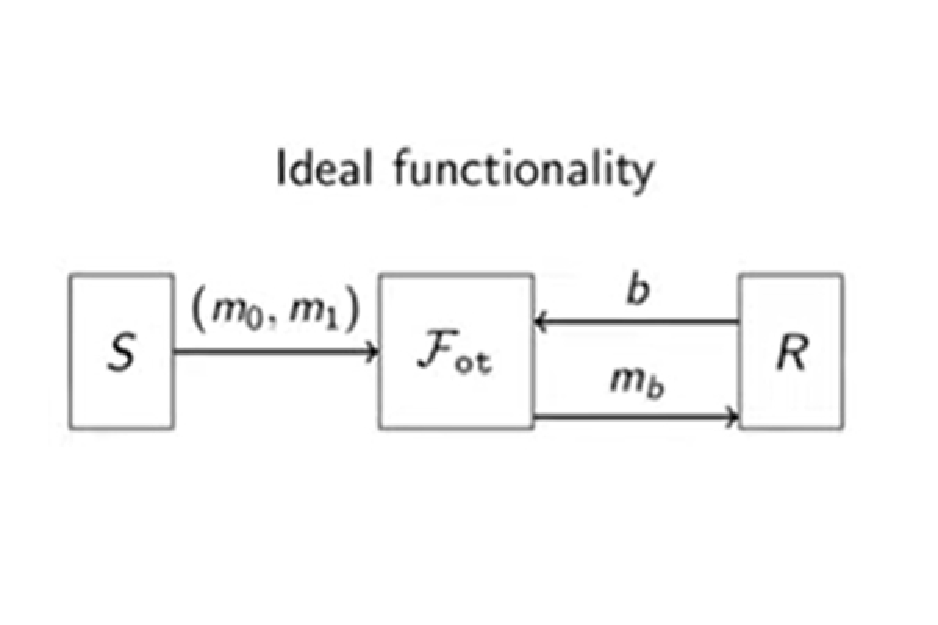
\includegraphics[width=\linewidth]{figures/images/img-5.pdf}
            \caption{An Oblivious Transfer (OT)\\ protocol in the ideal world.}
            \label{fig:oblivious-transfer-protocol-ideal-world}
        \end{subfigure}%
        \begin{subfigure}{.5\textwidth}
            \centering
            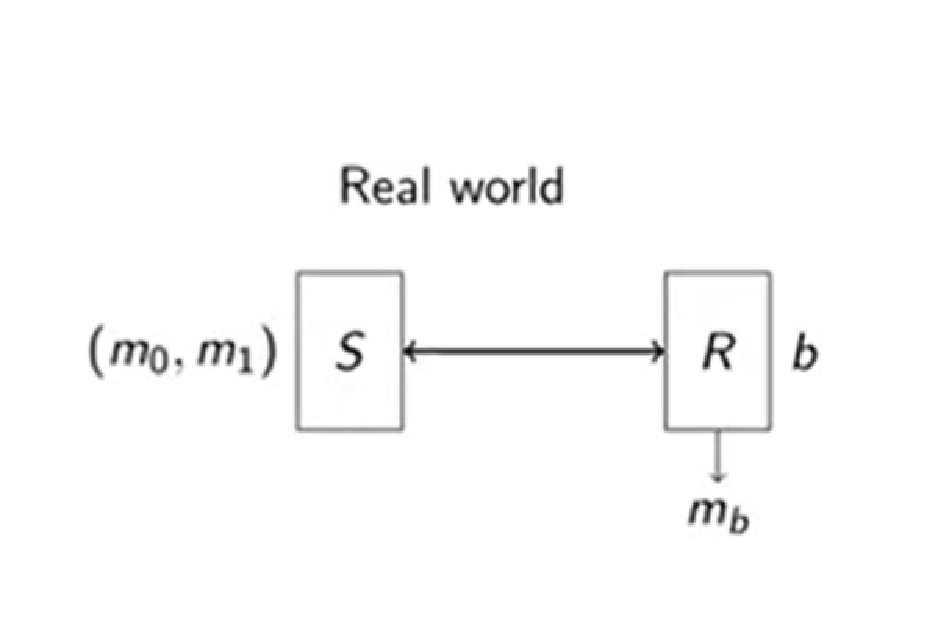
\includegraphics[width=\linewidth]{figures/images/img-6.pdf}
            \caption{An Oblivious Transfer (OT)\\ protocol in the real world.}
            \label{fig:oblivious-transfer-protocol-real-world}
        \end{subfigure}
        \caption{High-level illustration of an Oblivious Transfer (OT)\\ protocol in ideal and real worlds.}
        \label{fig:oblivious-transfer-protocol-ideal-and-real-worlds}
    \end{figure}

    \noindent Now, let's dive into some quantum protocols to perform this mentioned OT primitive. At the beginning times of Quantum Cryptography, Claude Cr\'{e}peau and Joe Kilian proposed the Cr\'{e}peau-Kilian-1988 (CK88) protocol\break \cite{crepeau-kilian:achieving-oblivious-transfer-using-weakened-security-assumptions:1988:03-2024,crepeau-kilian:weakening-security-assumptions-and-oblivious-transfer:1988:03-2024} in 1988, as well as Charles Bennett, Gilles Brassard, Claude Cr\'{e}peau and Marie-H\'{e}l\`{e}ne Skubiszewska together proposed a similar protocol in 1992, known as Bennett-Brassard-Cr\'{e}peau-Skubiszewska-1992 (BBCS92) protocol \cite{bennett-brassard-crepeau-skubiszewska:practical-quantum-oblivious-transfer:1992-03-2024}, which are two QOT protocols based on Commitment schemes,\break initially without real security proofs, which only appeared some years later \cite{damgard-fehr-lunemann-salvail-schaffner:improving-security-quantum-protocols-commit-and-open:2009:03-2024,bouman-fehr:sampling-quantum-population-and-applications:2012:03-2024}. Despite these Commitment schemes being simple cryptographic primitives, once we build them from weak assumptions, we need much stronger schemes to prove the security of QOT protocols, which we cannot construct\break from simple assumptions, such as One-Way Functions (OWFs). Namely, the first security proofs for these two quantum protocols only appeared in the XXI century, based on classical Commitment schemes, likely to lie outside the MiniCrypt paradigm \cite{impagliazzo:personal-view-average-case-complexity:1995:03-2024}, where lies every cryptographic primitive we can build from OWFs but where we do not expect MPC protocols to be \cite{impagliazzo-rudich:limits-provable-consequences-one-way-permutations:1990:03-2024,rudich:use-interaction-public-cryptosystems:1992:03-2024,impagliazzo:personal-view-average-case-complexity:1995:03-2024}. More recently, the first QOT protocols for strong Commitment schemes from OWFs emerged, such as the BCKM21 protocol \cite{bartusek-coladangelo-khurana-ma:one-way-functions-imply-secure-computation-quantum-world:2020:03-2024}, proposed by James\break Bartusek, Andrea Coladangelo, Dakshita Khurana, and Fermi Ma, as well as\break the GLSV21 protocol \cite{grilo-lin-song-vaikuntanathan:oblivious-transfer-miniqcrypt:2020:03-2024}, proposed together by Alex Grilo, Huijia Lin, Fang Song, and Vinod Vaikuntanathan, both dated from 2021. The main point now is that we know how to build QOT protocols, as well as how to build OT\break protocols classically from strong assumptions. These recent research results\break showed us how to construct these Commitment schemes needed in\break the security proofs for quantum protocols from OWFs. We often consider OWFs the classical minimal assumption in these security proofs since we\break cannot perform computational cryptography with OWFs classically. These research results show that we can build these quantum MPC protocols on what we can call MiniQCrypt paradigm \cite{grilo-lin-song-vaikuntanathan:oblivious-transfer-miniqcrypt:2020:03-2024}, a variant of the MiniCrypt paradigm that uses quantum phenomena and minimal classical primitives. Therefore, this ends up giving us some interesting results in terms of\break computational complexity, in a natural sense that it is not possible to build MPC protocols only from OWFs, and we need this strong separation between quantum and classical resources on top of OWFs. Furthermore, between\break the '80s and the '90s, the research community thought we could build\break Commitment schemes with unconditional security only with quantum\break resources \cite{brassard-crepeau-jozsa-langlois:quantum-bit-commitment-scheme-provably-unbreakable-both-parties:1993:03-2024,brassard-crepeau:25-years-quantum-cryptography:1996:03-2024,crepeau:what-going-wrong-quantum-bit-commitment:1996:03-2024,mayers:unconditional-secure-quantum-bit-commitment-impossible:1997:03-2024,brassard-crepeau-mayers-salvail:brief-review-impossibility-quantum-bit-commitment:1997:03-2024,lo-chau:why-quantum-bit-commitment-ideal-quantum-coin-tossing-impossible:1998:03-2024,brassard-crepeau-mayers-salvail:defeating-classical-bit-commitments-quantum-computer:1998:03-2024,kent:quantum-bit-commitment-from-computation-bound:1999:03-2024,kent:permanently-secure-quantum-bit-commitment-temporary-computation-boud:1999:03-2024}. But later on, a few security proofs appeared saying we could not achieve that, and we always need to consider some additional\break classical minimal assumptions for these types of quantum protocols.
    
    \section{CK88/BBCS92 Protocols}
    \label{sec:ck88-bbcs92-protocols}
    
    In the CK88/BBCS92 protocol(s) \cite{crepeau-kilian:achieving-oblivious-transfer-using-weakened-security-assumptions:1988:03-2024,crepeau-kilian:weakening-security-assumptions-and-oblivious-transfer:1988:03-2024,bennett-brassard-crepeau-skubiszewska:practical-quantum-oblivious-transfer:1992-03-2024}, we have two parties as usually\break happens in a two-party quantum cryptographic protocol with $\lambda$ rounds, namely the sender (e.g., Alice) and the receiver (e.g., Bob). The sender starts by picking a specific quantum state, such as the Bennett-Brassard-1984\break (BB84) state \cite{bennett-brassard:quantum-cryptography-public-key-distribution-coin-tossing:1984:03-2024,bennett-brassard:quantum-cryptography-public-key-distribution-coin-tossing:2014:03-2024}. Then, the sender needs to pick a random bit string $\vec{x}$ (i.e., a string containing bits with the values $0$s a $1$s) of size $\lambda$ in this case and a random bases list $\vec{\theta}$ (i.e., $\mathbb{X}$ and $\mathbb{Z}$ basis, for each round) of size $\lambda$ to encode each one of those bits in a quantum state randomly prepared accordingly (i.e., $|0\rangle$, $|+\rangle$, $|1\rangle$, and $|-\rangle$, for each round) and send them to the receiver. On the other side, the receiver also picks a random bases list $\vec{\hat{\theta}}$ (i.e., $\mathbb{X}$ and $\mathbb{Z}$ basis, for each round) of size $\lambda$, measuring each one of the corresponding incoming\break quantum states on the respective randomly chosen basis, obtaining some\break resulting outcome list $\vec{\hat{x}}$, in the form of bits (i.e., $0$s and $1$s). Then, the sender sends the list $\vec{\theta}$ of bases randomly chosen to the receiver, who can split the outcomes information into two sets: the set where the bases randomly\break picked by both parties match between them and the set where those bases do not match. Then, the receiver calls ${I}_{b} = \{ i: {\vec{{\theta}}}_{i} = {\vec{\hat{\theta}}}_{i} \}$ to the set where the bases match where $b$ is the classical bit they want to learn. This set ${I}_{b}$\break supposedly has the correct and completely correlated bits since the outcomes in these cases (i.e., the quantum states prepared and then measured on the same basis) are deterministic. On the other hand, each party has another set\break ${I}_{\bar{b}} = \{ i: {\vec{{\theta}}}_{i} \neq {\vec{\hat{\theta}}}_{i} \}$ where the randomly chosen bases do not match, and the resulting obtained outcomes in these cases will be completely random in\break the form of incorrect and totally uncorrelated bits. For the set of matching\break bases, for example, the receiver has all the same information the sender has.\break The receiver sends the two sets to the sender only in the form of\break the corresponding indices. By doing that, we should notice that the sender does not know which set contains the matching bases because the receiver sends the ${I}_{0}$ and ${I}_{1}$, and this does not tell us what the ${I}_{b}$ is for each case. Then, the sender prepares two messages ${m}_{0}$ and ${m}_{1}$, in the form of bit strings, and by using some sort of encryption, such as the Advanced Encryption\break Standard (AES) protocol \cite{rijmen-daemen:advanced-encryption-standard:2001:02-2024}, the sender encrypts the bits of those messages,\break using the bits corresponding to the indices of the initial randomly chosen bit string according to the sets ${I}_{b}$ as the keys of the encryptor for the two\break messages ${m}_{0}$ and ${m}_{1}$, resulting in the two sets ${a}_{0} = {Enc}_{{\vec{x}}_{{I}_{0}}}({m}_{0})$ and\break ${a}_{1} = {Enc}_{{\vec{x}}_{{I}_{1}}}({m}_{1})$. Then, the sender sends these two encrypted messages ${a}_{0}$ and ${a}_{1}$ to the receiver. From these two encrypted messages, the receiver\break should be able to correctly learn the content of one of the messages ${m}_{b}$ using\break the corresponding set of matching bases by performing the respective\break decryption ${m}_{b} = {Dec}_{{\vec{x}}_{{I}_{b}}}({a}_{b})$. However, there is a trivial security problem with these protocols, which is the receiver can decrypt both messages ${a}_{0}$ and ${a}_{1}$, if it has access to a bounded quantum memory, by keeping all the incoming\break quantum states in memory, waiting for the sender sending the randomly\break chosen bases used to prepare those quantum states, and then, being able to correctly measure all of them in the correct basis, obtaining the whole bit string randomly chosen by the sender, also obtaining both messages ${m}_{0}$ and ${m}_{1}$ at the end. This observation shows us that there are some security models\break where we assume the receiver has access to a bounded quantum memory, which makes these quantum protocols insecure. However, we want to be ``paranoid'' when building these security models and show that even malicious\break receivers with bounded quantum memory cannot cheat in this protocol.\break For this same reason, we need to add more cryptographic primitives to\break this quantum cryptographic protocol to force the receiver to measure always the incoming quantum states without keeping them in a quantum memory.

   \begin{figure}[ht]
        \captionsetup{justification=centering}
        \centering
        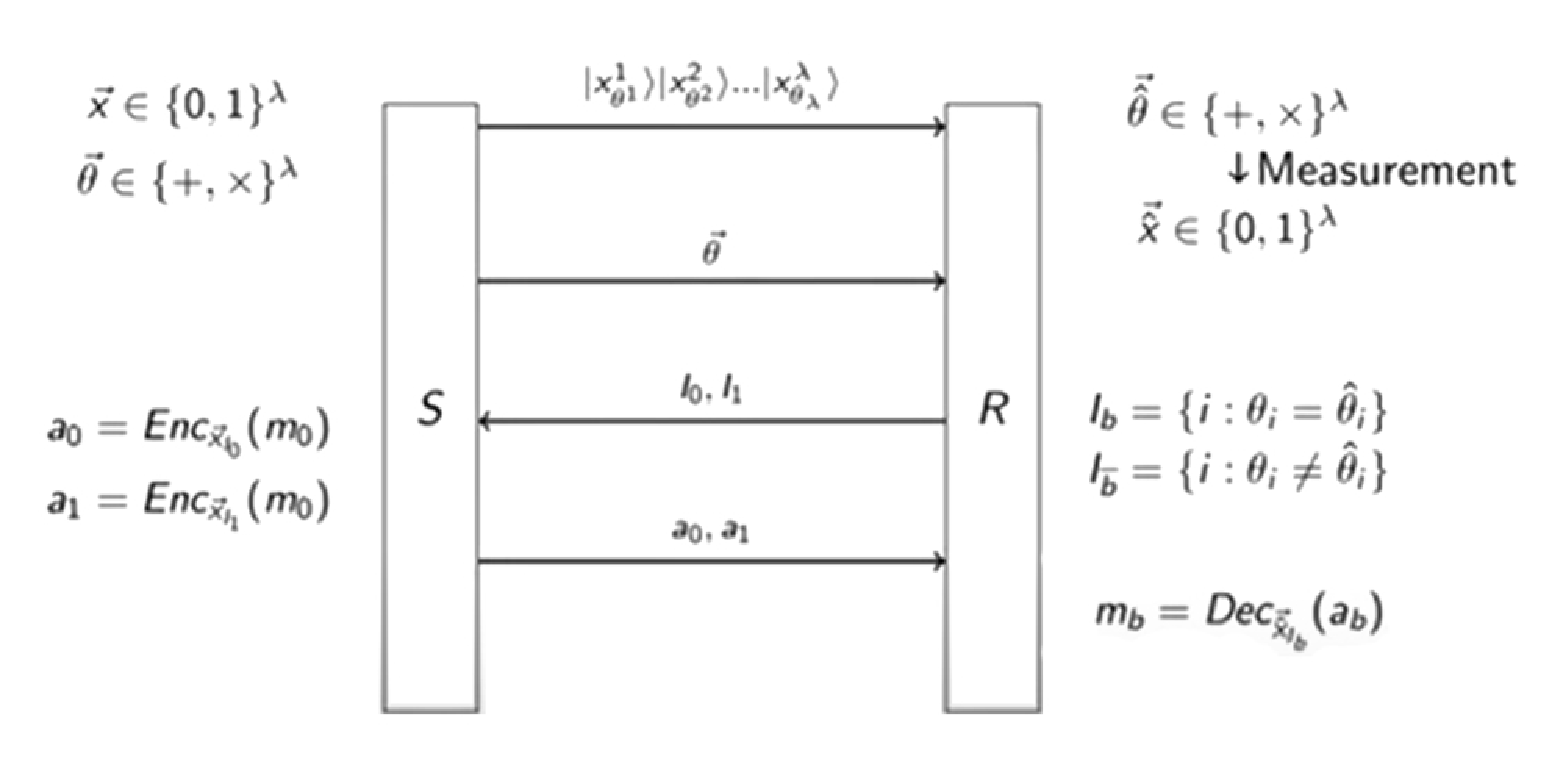
\includegraphics[width=0.8\textwidth]{figures/images/img-7.pdf}
        \caption{High-level illustration of both\\ the Cr\'{e}peau-Kilian-1988 (CK88) and Bennett-Brassard-Cr\'{e}peau-Skubiszewska-1992 (BBCS92)\\ protocols.}
        \label{fig:crepeau-kilian-1988-and-bennett-brassard-crepeau-skubiszewska-1992-protocols}
    \end{figure}
        
    \section{Quantum Bit-Commitment Schemes with Simulation Model for Security}
    \label{sec:quantum-bit-commitment-schemes-with-simulation-model-for-security}

    The cryptographic primitive we need as a solution for this last-mentioned security flaw is a Bit Commitment scheme. This cryptographic scheme is a two-phase protocol, where we still have two parties again: the sender, acting also as the committer of the protocol, and the receiver. In the first phase of the protocol, the committer has a message $m$, and it wants to commit to the value or content of this same message in a way that the sender and receiver exchange some message(s), and by the end, the receiver should obtain the commitment of this message $m$. In the second phase of the protocol, the committer will finally open this message $m$. Then, we want to ensure two properties for the correctness of this protocol. First, we want to ensure that the receiver should not be able to learn what the message really is during the first phase of the protocol, in a property usually called \textit{hiding}. Second, we want to ensure that the committer cannot change its mind and choose to open a different message, and due to that, the commitment of $m$ should fix this message $m$, in a property we usually call \textit{biding}. However, for Cryptography\break in general, we have several different types of security requirements, and these \textit{hiding} and \textit{biding} properties are known as the ``vanilla'' commitment\break requirements. But, there are other fencer ways of defining these commitment requirements and properties, such as by the well-known simulation model.

   \begin{figure}[ht]
        \captionsetup{justification=centering}
        \centering
        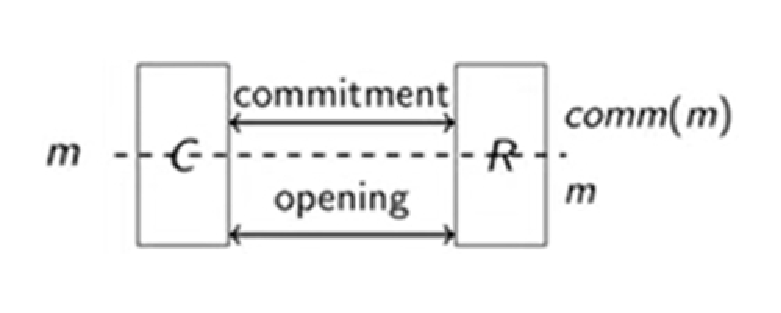
\includegraphics[width=0.5\textwidth]{figures/images/img-8.pdf}
        \caption{High-level illustration of\\ the Simulation Security Model of the Bit-Commitment protocols.}
        \label{fig:simulation-security-model-bit-commitment-protocols}
    \end{figure}

    \noindent There is a simulation version of the \textit{hiding} property called \textit{equivocality} and a simulation version of the \textit{biding} property called \textit{extractability}. These two mentioned simulation variants of properties are the ones we morally need in this previous result that proves the security of the QOT protocol. 
    
    \begin{figure}[ht]
        \captionsetup{justification=centering}
        \centering
        \begin{subfigure}{.5\textwidth}
            \centering
            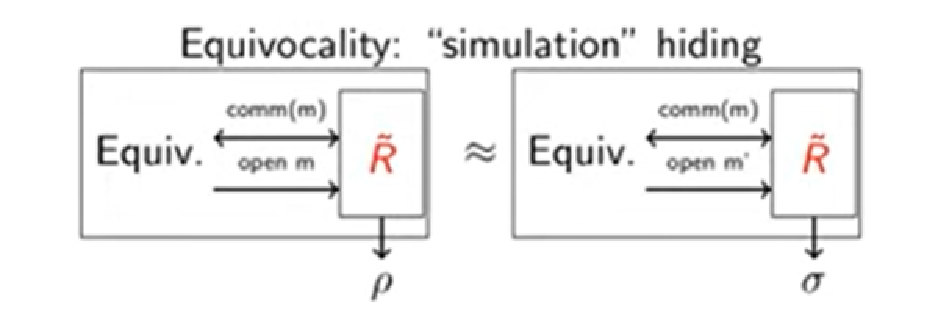
\includegraphics[width=\linewidth]{figures/images/img-9.pdf}
            \caption{Simulated version of \textit{Hiding} property: \textit{Equivocality}.}
            \label{fig:simulated-version-hiding-property-equivocality}
        \end{subfigure}%
        \begin{subfigure}{.5\textwidth}
            \centering
            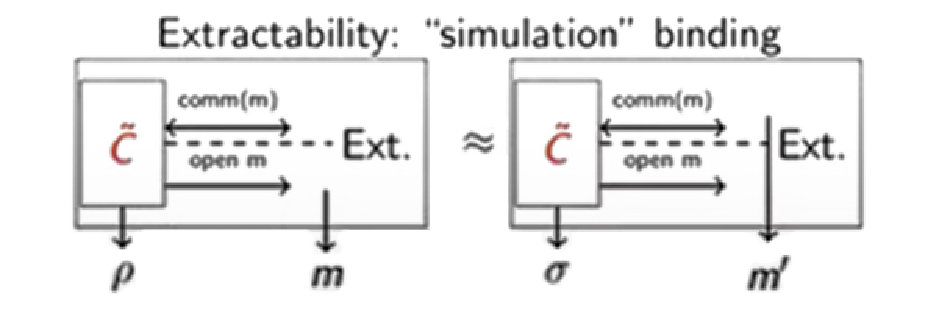
\includegraphics[width=\linewidth]{figures/images/img-10.pdf}
            \caption{Simulated version of \textit{Biding} property: \textit{Extractability}.}
            \label{fig:simulated-version-biding-property-extractability}
        \end{subfigure}
        \caption{Simulated versions of the \textit{Hiding} and \textit{Biding}\\ security properties: \textit{Equivocality} and \textit{Extractability}.}
        \label{fig:simulated-versions-hiding-and-biding-properties-equivocality-and-extractability}
    \end{figure}
    
    \noindent Therefore, going back to the description of the QOT protocol, the idea is that we can add some additional steps to force the receiver to measure\break the incoming quantum states as soon as it receives them, making the protocol\break more secure. In order to achieve that, the receiver will commit to the pair with the randomly chosen basis and the resulting measurement outcome in each round $1 \leq i \leq \lambda$, sending this commitment pair ${c}_{i} = comm( {\hat{\theta}}_{i}, {\hat{x}}_{i} )$ to the sender. Then, the sender can pick just a random subset of indices $T$ and ask the receiver to open the commitment pairs ${c}_{i}$ for the rounds\break corresponding to those indices $i \in T$. Namely, for the committed rounds where the randomly chosen bases match, the sender can verify if the outcomes are the same as expected. If we choose a big enough set $T$ and perform enough testing rounds, we can have some guarantees that, even if the receiver does not measure all the corresponding quantum states, it had to have measured a lot of those quantum states to pass a pre-defined commitment test. After\break all the committed pairs are verified, the sender and the receiver can discard them. If the receiver has measured several quantum states corresponding to\break those committed pairs and passed the commitment test, we have guarantees\break that the receiver cannot decrypt both messages. And if we can ensure the receiver cannot decrypt both messages ${m}_{0}$ and ${m}_{1}$, we have what is necessary to prove the security of the QOT protocol in this case. Obviously, we need more formal security proof for this situation, but this is the intuition why we end up forcing the receiver to measure the incoming quantum states as soon as they arrive at its side by having this commitment verification. After\break performing this additional step of commitment verification, both parties\break continue the execution of the QOT protocol with the not discarded rounds.

   \begin{figure}[ht]
        \captionsetup{justification=centering}
        \centering
        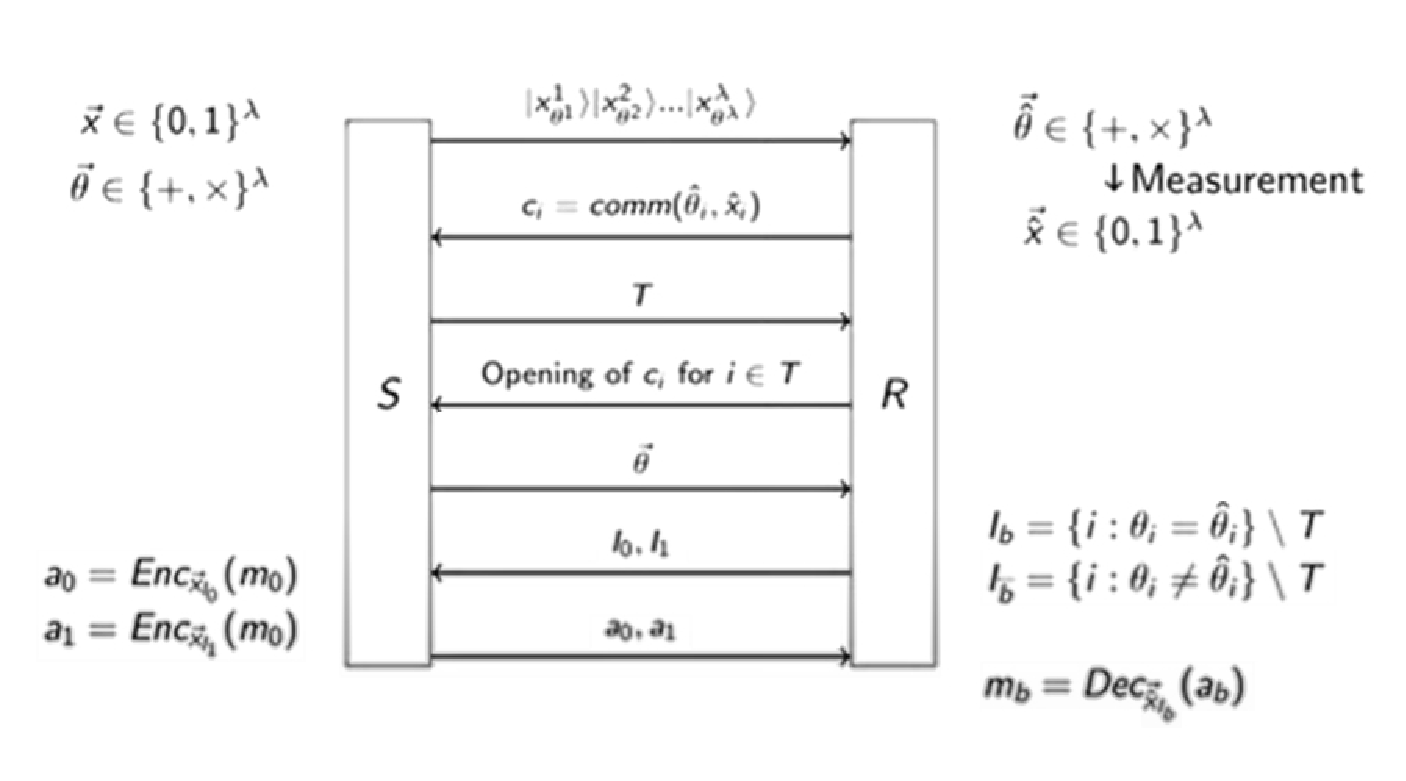
\includegraphics[width=0.8\textwidth]{figures/images/img-11.pdf}
        \caption{High-level illustration of\\ the Quantum Oblivious Transfer (QOT) CK88/BBCS92 protocol(s)\\ based on a Bit-Commitment scheme.}
        \label{fig:quantum-oblivious-transfer-ck88-bbcs92-protocols-based-bit-commitment-scheme}
    \end{figure}

    \noindent Obviously, we also need to consider the cases in which the simulator pretends to have committed to a measured quantum state but then changes its mind to prove security for the hiding property of the simulation model.
    
    \noindent This scheme represents the security proof for the simulation model, using the \textit{equivocality} property, allowing us to prove security against malicious senders:

   \begin{figure}[ht]
        \captionsetup{justification=centering}
        \centering
        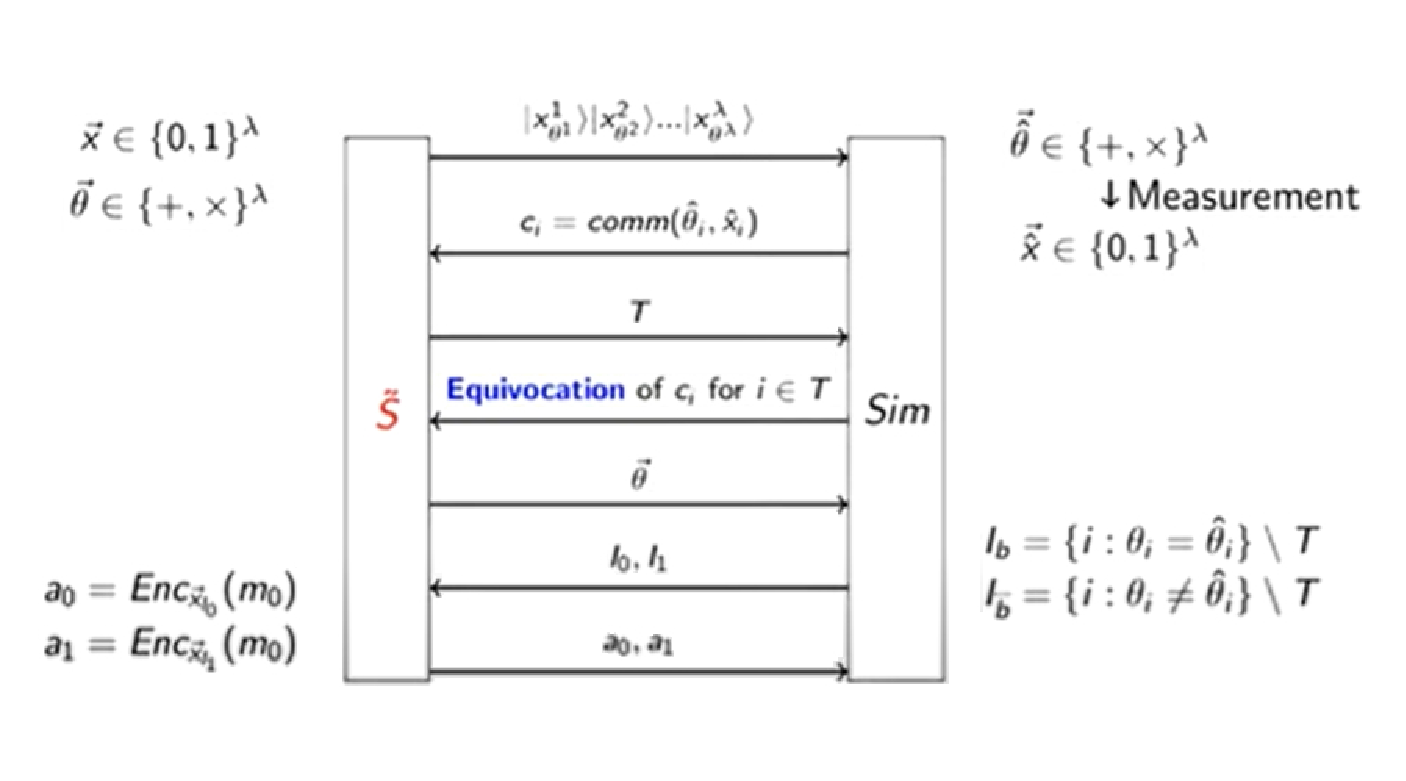
\includegraphics[width=0.74\textwidth]{figures/images/img-12.pdf}\phantom{...................}\\
        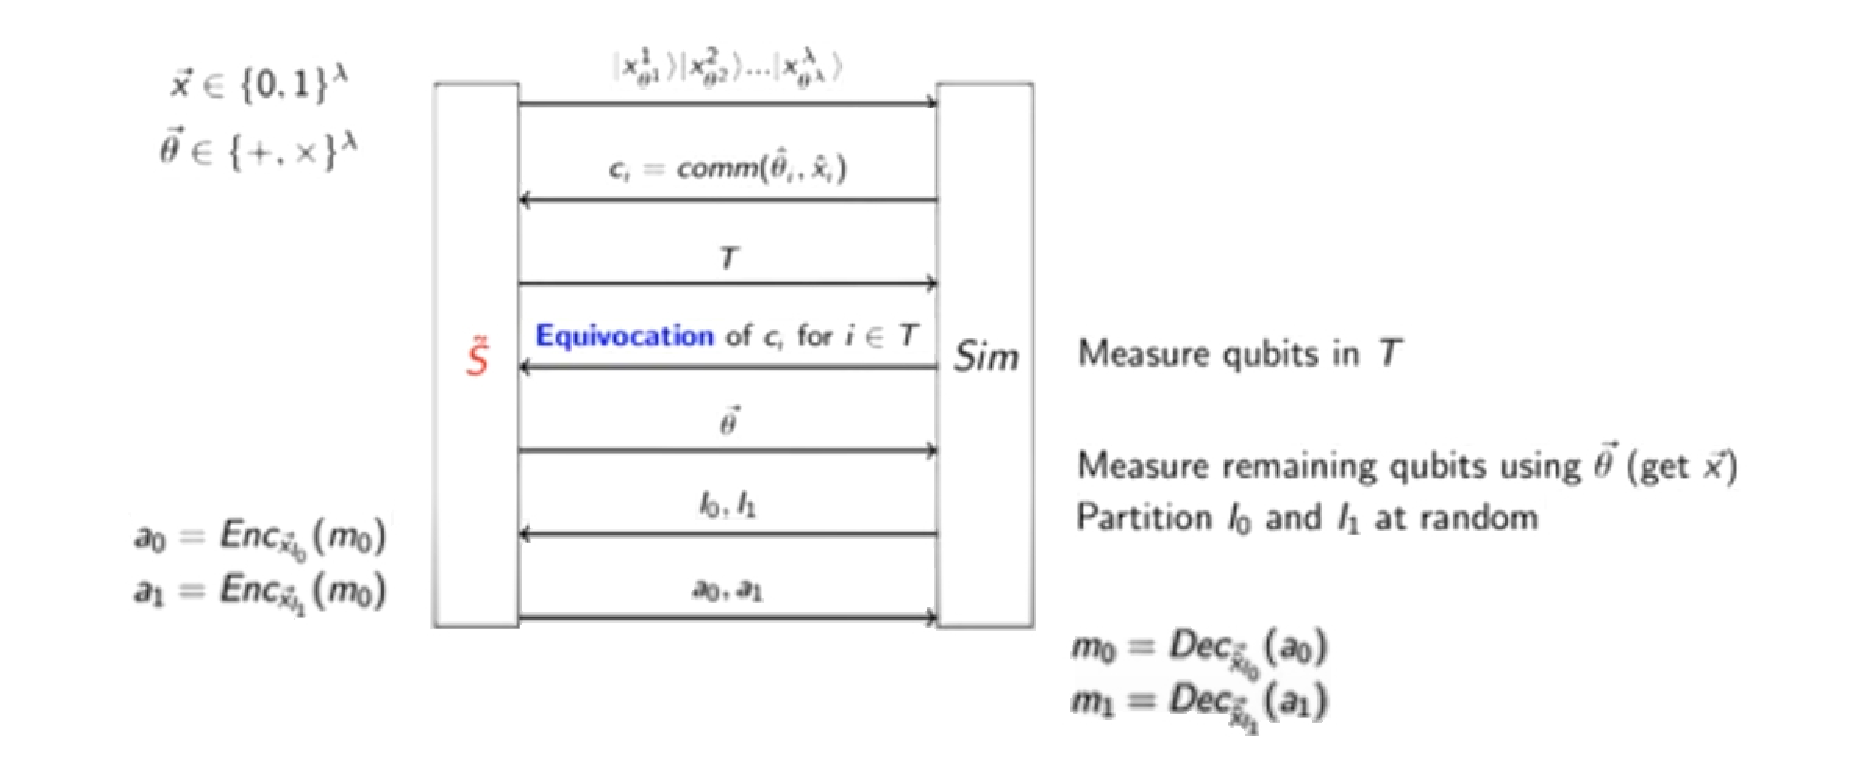
\includegraphics[width=\textwidth]{figures/images/img-13.pdf}
        \caption{High-level illustration of\\ the simulated \textit{Equivocality} security property for\\ the Quantum Oblivious Transfer (QOT) CK88/BBCS92 protocol(s)\\ based on a Bit-Commitment scheme.}
        \label{fig:simulated-equivocality-security-property-quantum-oblivious-transfer-ck88-bbcs92-protocols-based-bit-commitment-scheme}
    \end{figure}

    \clearpage
    
    \noindent On the other hand, this representative scheme represents the security proof for the simulation model, using the \textit{extractability} property, which allows us to prove security against malicious receivers trying to learn both messages:

   \begin{figure}[ht]
        \captionsetup{justification=centering}
        \centering
        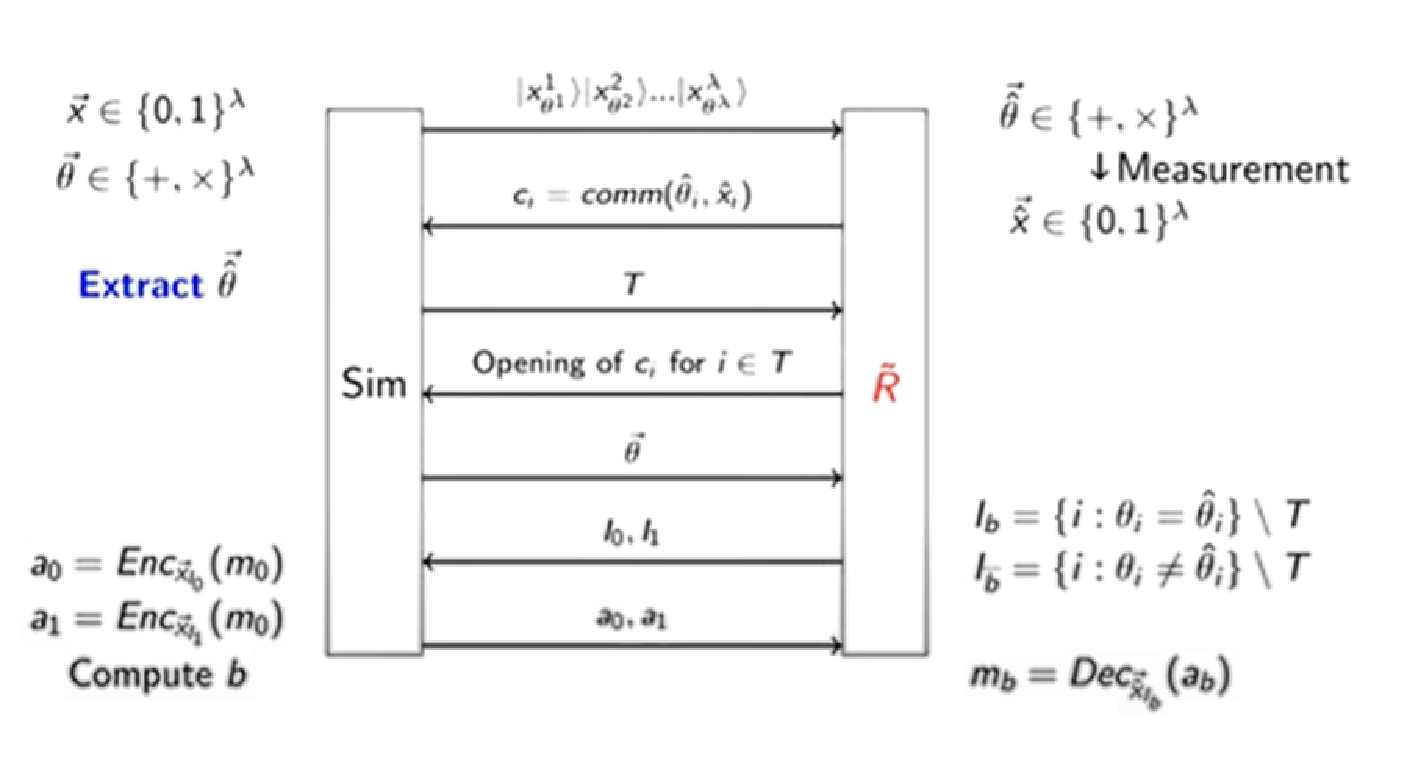
\includegraphics[width=0.8\textwidth]{figures/images/img-14.pdf}
        \caption{High-level illustration of\\ the simulated \textit{Extractability} security property for\\ the Quantum Oblivious Transfer (QOT) CK88/BBCS92 protocol(s)\\ based on a Bit-Commitment scheme.}
        \label{fig:simulated-extractability-security-property-quantum-oblivious-transfer-ck88-bbcs92-protocols-based-bit-commitment-scheme}
    \end{figure}

    \noindent Then, we can use these two previously mentioned research results related to security proofs of BCKM21 \cite{bartusek-coladangelo-khurana-ma:one-way-functions-imply-secure-computation-quantum-world:2020:03-2024} and GLSV21 \cite{grilo-lin-song-vaikuntanathan:oblivious-transfer-miniqcrypt:2020:03-2024} QOT protocols, for which the main goal is also to implement these Commitment schemes with the \textit{hiding} and \textit{biding} properties for the security model with Simulation. Namely, we can also use LWE problems to achieve these OT protocols based on Commitment schemes, for example. These two results showed us how to build these Commitment schemes using quantum protocols and having these hiding and biding properties. Actually, these two quantum protocols use OT as a bootstrap to achieve a Commitment scheme. Therefore, we take inspiration from both work proposals, and we can use the CK88 protocol \cite{crepeau-kilian:achieving-oblivious-transfer-using-weakened-security-assumptions:1988:03-2024,crepeau-kilian:weakening-security-assumptions-and-oblivious-transfer:1988:03-2024} with a weak commitment to obtain a Commitment scheme and then use this protocol again to achieve a full QOT protocol. The main differences

    \clearpage
    
    \noindent between BCKM21 \cite{bartusek-coladangelo-khurana-ma:one-way-functions-imply-secure-computation-quantum-world:2020:03-2024} and GLSV21 \cite{grilo-lin-song-vaikuntanathan:oblivious-transfer-miniqcrypt:2020:03-2024} QOT protocols are given below:

    \begin{table}[htp]
        \centering
        \begin{tblr}{
            width = \linewidth,
            colspec = {Q[425]Q[515]},
            cells = {c},
            cell{1}{1} = {c=2}{0.94\linewidth},
            cell{3}{1} = {c=2}{0.94\linewidth},
            cell{5}{1} = {r=2}{},
            cell{7}{1} = {c=2}{0.94\linewidth},
            vlines,
            hline{1-5,7-10} = {-}{},
            hline{6} = {2}{},
            }
            \textbf{Protocols} ~ ~ ~ ~ ~ & \\
            \textbf{BCKM21} \cite{bartusek-coladangelo-khurana-ma:one-way-functions-imply-secure-computation-quantum-world:2020:03-2024} & \textbf{GLSV21} \cite{grilo-lin-song-vaikuntanathan:oblivious-transfer-miniqcrypt:2020:03-2024}\\
            \textbf{Specifications} ~ ~ ~ ~ ~ & \\
            {1. (Black-Box)\\ Equivocality Compiler} & {1. Equivocal Commitment from\\ Naor's Commitment Scheme \cite{naor:bit-commitment-using-pseudorandomness:1991:03-2024} and\\Zero-Knowledge Proofs (ZKPs) \cite{goldwasser-micali-rackoff:1985:03-2024,fiat-shamir:how-prove-yourself-practical-solutions-identification-signature-problems:1987:03-2024,blum-feldman-micali:non-interactive-zero-knowledge-applications:1988:03-2024}}\\
            {2. Extractable\\ Commitment scheme from\\Equivocal Bit-Commitment and Quantum Communication} & {2. Unbounded-Simulator\\ Oblivious Transfer (OT) protocol from\\ Equivocal Commitment}\\
            & {3. Extractable and Equivocal Bit-Commitment scheme from\\ Unbounded-Simulator\\ Oblivious Transfer (OT) protocol and\\ Quantum Communication}\\
            \textbf{Features} ~ ~ ~ ~ ~ & \\
            {\textbf{Black-Box} use of\\ One-Way Functions (OWFs)} & {\textbf{Constant-Round}\\ Oblivious Transfer (OT) protocol in\\ the Common Reference String (CRS) Model \cite{canetti-fischlin:universally-composable-commitments:2001:03-2024}}\\
            \textbf{Statistical} Security against Malicious Receiver & \textbf{Statistically Binding} Extractable Bit-Commitment Scheme
        \end{tblr}
    \end{table}

    \noindent In an experimental ``toy'' scenario, let's consider we have two parties, the sender (Alex) and the receiver (Eleni), who start a conversation before the start of the protocol. The sender wants to tell the receiver it has a QOT protocol that only uses BB84 states. Thus, the only thing the sender has to send in this QOT protocol is BB84 states, and the receiver has to measure them, as happens in Quantum Key Distribution (QKD) protocols. Then, the parties agree on implementing this quantum protocol, and the conversation\break continues. The receiver asks the sender how much noise this protocol can\break tolerate, and the sender says there will be no noise in the quantum\break communication channel. Then, the receiver asks how many quantum states the sender will need to send, and the sender replies that it will need to send $poly(\lambda)$ quantum states. After that, the receiver asks the sender what is this $\lambda$ variable, to which the sender replies that it is the security parameter. Next, the receiver asks the sender how many bits of security will be achieved in this protocol since they are talking about a concrete implementation, to which the sender replies again that it will be $poly(\lambda)$. Finally, the receiver asks the sender about the requirements and complexity of classical post-processing, to which the sender replies that it has no idea how to implement it in practice.
    
   \begin{figure}[ht]
        \captionsetup{justification=centering}
        \centering
        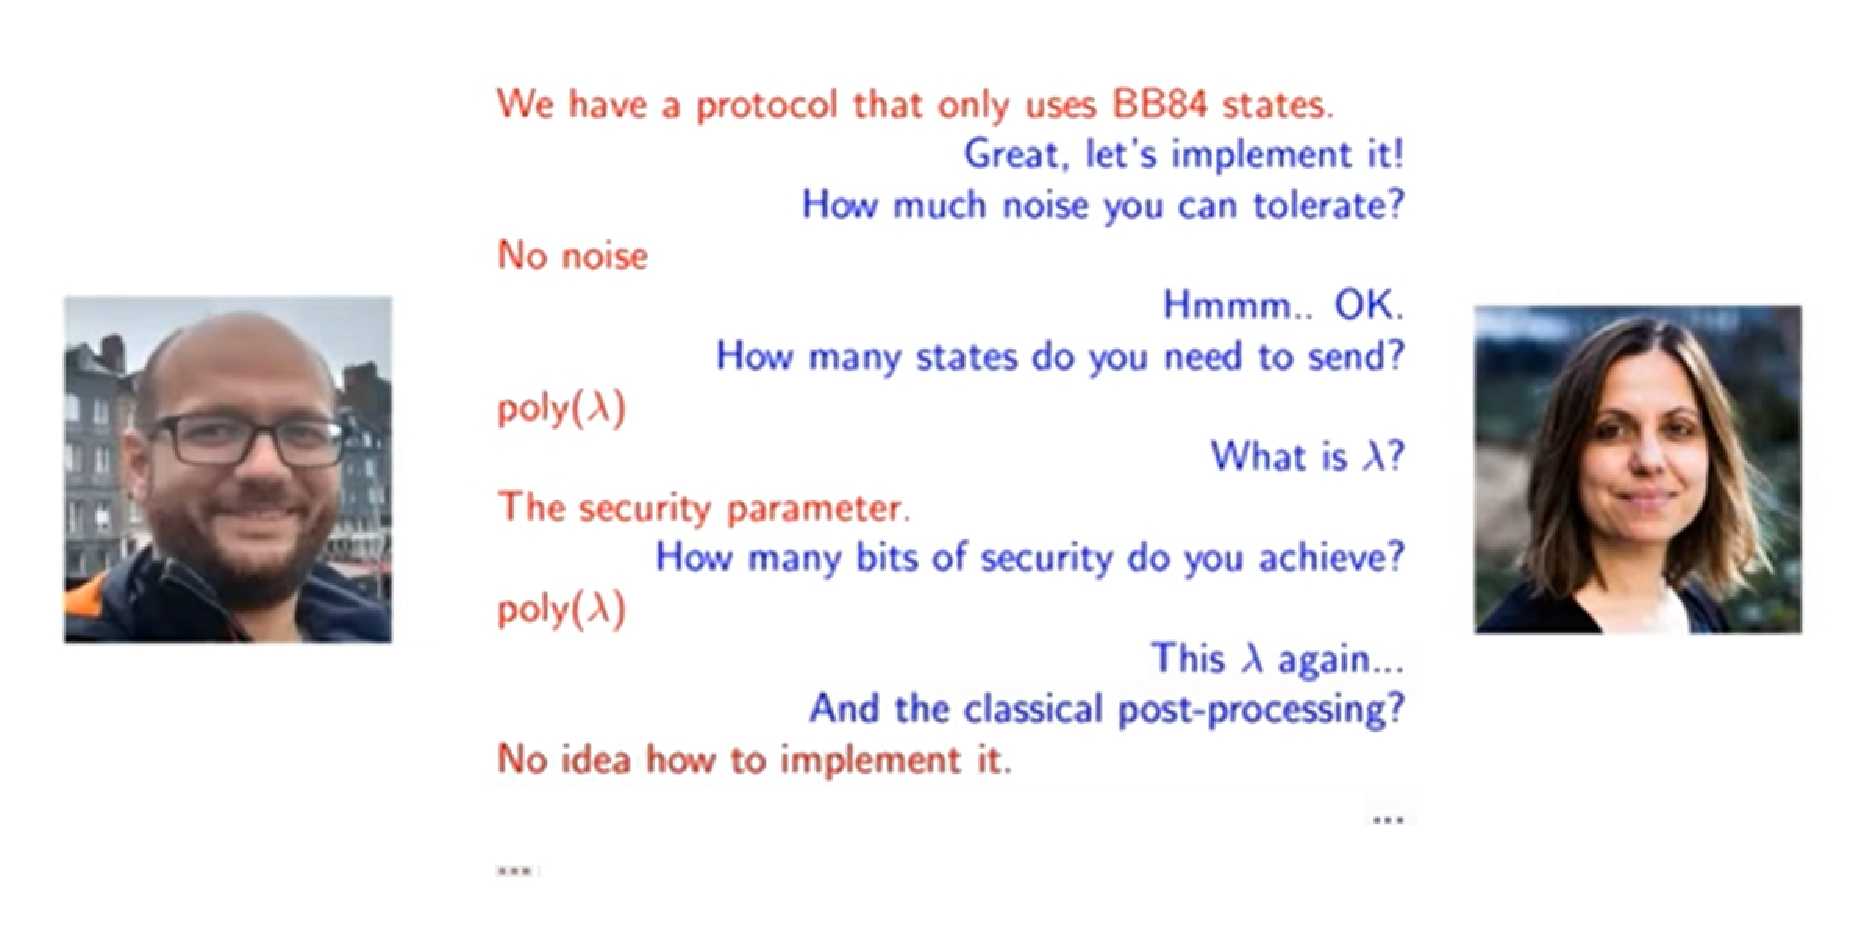
\includegraphics[width=\textwidth]{figures/images/img-15.pdf}
        \caption{Experimental ``toy'' scenario for the setup of\\ a QOT protocol based on a Bit-Commitment scheme.}
        \label{fig:experimental-toy-scenario-setup-quantum-oblivious-transfer-protocol-based-bit-commitment-scheme}
    \end{figure}

    
    \section[Practical Implementation of QOT Protocols from OWFs]{Practical Implementation of\\ QOT Protocols from OWFs}
    \label{sec:practical-implementation-qot-protocols-from-owfs}

    In order to implement this QOT protocol from OWF, we need to send these BB84 quantum states, which seems to imply the use of basic technology for QKD protocols. However, there are several reasons to assume a perfect\break creation/transmission/measurement of the quantum states in these quantum\break cryptographic protocols. Some of the physical apparatus we use for these\break quantum protocols are easy to fix if they fail, but some of them do not. These quantum cryptographic protocols rely on complicated classical primitives.\break For example, the author highlights a quantum protocol developed with his team and based on ZKPs with great theoretical results, on which we can\break obtain ZKPs for all Nondeterministic Polynomial-time (NP) statements. But when we have a concrete language we want to prove using that protocol, we might be required to perform and implement a complicated reduction. In that case, the author's team usually avoids it and implements a different quantum\break protocol since translating asymptotic security to concrete cases is hard,\break especially in the quantum setting. From these previous theoretical results,\break we also know that, in theory, we need to repeat poly rounds on the protocol.\break However, we also want to know how many bits of security we achieve at the end, for which we need to be precise on the respective calculations that are hard. Therefore, the goal of the author and his team, is to push these\break quantum cryptographic protocols from theory to practice. Several interesting\break theory questions come out from these types of experiments. The goal of\break the author and his team is not to design new quantum cryptographic\break protocols from scratch but to consider some parts of the protocols and\break redesign them to be more memory efficient, for example. In that direction, they are focusing more on experimental and practical problems. One of the focuses of these tasks is to redesign the quantum cryptographic protocols to account for noise and to save classical memory since one of the problems of quantum cryptographic protocols for the latter case is that they require a lot of classical memory for classical post-processing. After redesigning these quantum protocols, the author and his team do not want to prove the security only from an abstract point of view, but also want to figure out how many quantum states are sending and how many bits of security they obtain at the end, by reproving the security of the protocols asymptotically and with concrete parameters. Finally, the author and his team want to physically implement and test these quantum cryptographic protocols in the lab, as in a real scenario where we have two real parties, impersonating Alice and Bob.

    
    \section{Open Questions}
    \label{sec:open-questions}

    In this seminar, the author addressed some aspects of MPC protocols, but we should also think about some open questions and future work. For example, we can think about what else we can achieve on top of MPC or OT protocols with quantum resources and OWFs, usually as happens in the MiniQCrypt paradigm. We should also think about what (black-box) separations exist for cryptographic primitives in the quantum setting and MiniQCrypt paradigm. Another direction we can follow is to show what we cannot achieve by\break building cryptographic protocols with quantum resources and OWFs. There are other interesting partial research results proposed recently on building\break new quantum cryptographic primitives from weaker assumptions than\break OWFs, such as Pseudo-Random Quantum States (PRQS) \cite{ji-liu-song:pseudorandom-quantum-states:2018:03-2024,ananth-qian-yuen:cryptography-pseudorandom-quantum-states:2022-03-2024} or even\break Efficient-Far-Indistinguishable (EFI) pairs of quantum states \cite{yan:general-properties-quantum-bit-commitments:2020:03-2024,brakerski-canetti-qian:computational-hardness-needed-quantum-cryptography:2022:03-2024,morimae-yamakawa:one-wayness-quantum-cryptography:2022:03-2024}. On the other hand, we can think about which assumptions we can consider from the quantum world that could be weaker than OWFs, maybe unveilling a new paradigm. Finally, we can also think about other more practical new quantum cryptographic protocols or what we should do to transform the existing quantum cryptographic primitives on more practical variants.
    
    
    \bibliographystyle{unsrt}

    \clearpage
    
    \bibliography{bibliography}
    \label{bib:bibliography}
    
\end{document}